
\section{Study of Parallel Workload~\Rmnum{1}}
%\section{Identify the ``Bully"}
\label{sec:workload-1}

The study of Workload~\Rmnum{1} consists of two parts. First, we analyze the overall network performance when Workload~\Rmnum{1} is running under different placement and routing configurations. Second, we isolate each application from the workload and analyze its performance on both a per-rank basis as well as by considering router traffic resident to application ranks. The analysis allows us to identify the ``bully'' in Workload~\Rmnum{1}.

%\TODO{Add in a few words across the section (not here) on how previous work compares as you go through the results.}

\subsection{Network Performance Analysis}
\label{sec: workload-1 network analysis}

We first study the network performance at the system level by analyzing the degree of traffic and saturation seen at each router.

\begin{figure*}[t!]
    \centering
    \begin{subfigure}[t]{0.32\textwidth}
        \centering
        \includegraphics[height=1.8 in]{wkld/gc-traffic}
        \caption{Global Channel Traffic}
        \label{fig:global-channel-traffic}
    \end{subfigure}\hfill
    \hspace{1em}%
    \begin{subfigure}[t]{0.32\textwidth}
        \centering
        \includegraphics[height=1.8 in]{wkld/lc-traffic}
        \caption{Local Channel Traffic}
        \label{fig:local-channel-traffic}
    \end{subfigure}\hfill
    \hspace{1em}%
    \begin{subfigure}[t]{0.32\textwidth}
        \centering
        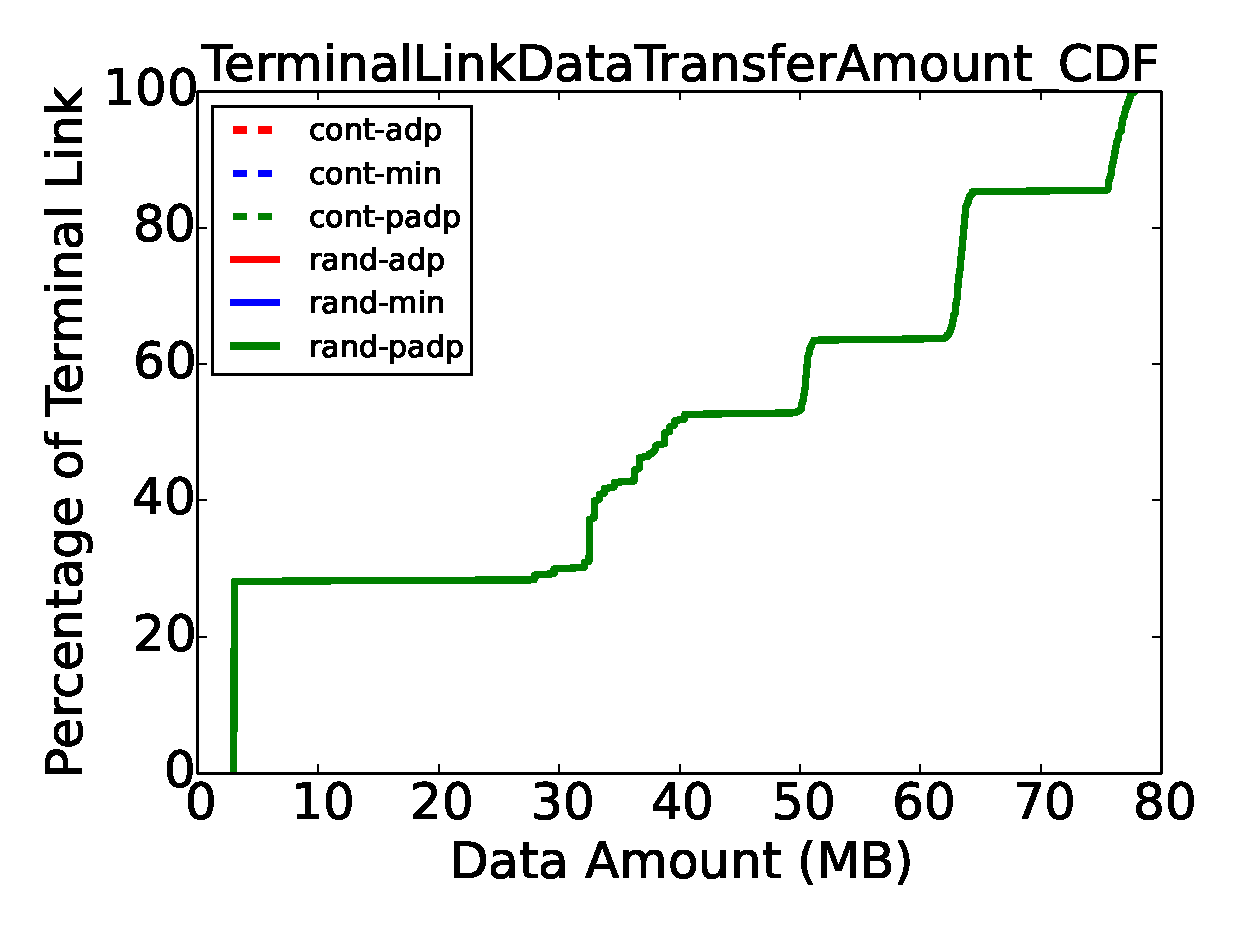
\includegraphics[height=1.8 in]{wkld/tl-traffic}
        \caption{Terminal Link Traffic}
        \label{fig:terminal-link-traffic}
    \end{subfigure}\\

    \centering   
    \begin{subfigure}[t]{0.32\textwidth}
        \centering
        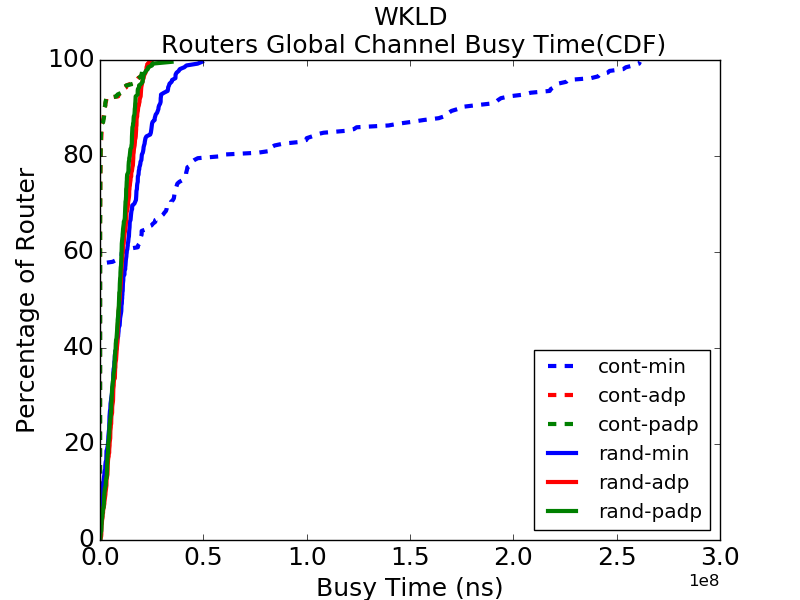
\includegraphics[height=1.8 in]{wkld/gc-stime}
        \caption{Global Channel Saturation Time}
        \label{fig:global-channel-stime}
    \end{subfigure}\hfill
     \hspace{1em}%
    \begin{subfigure}[t]{0.32\textwidth}
        \centering
        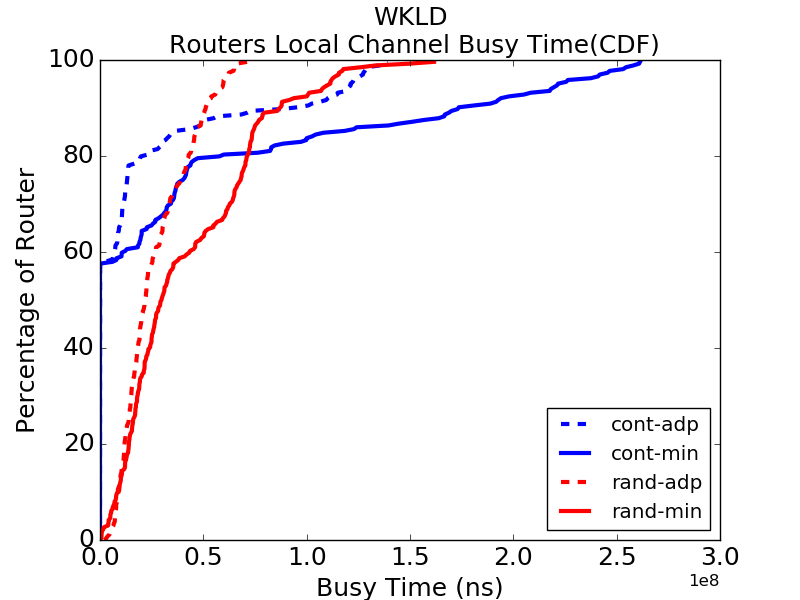
\includegraphics[height=1.8 in]{wkld/lc-stime}
        \caption{Local Channel Saturation Time}
        \label{fig:local-channel-stime}
    \end{subfigure}\hfill
    \hspace{1em}%
    \begin{subfigure}[t]{0.32\textwidth}
        \centering
        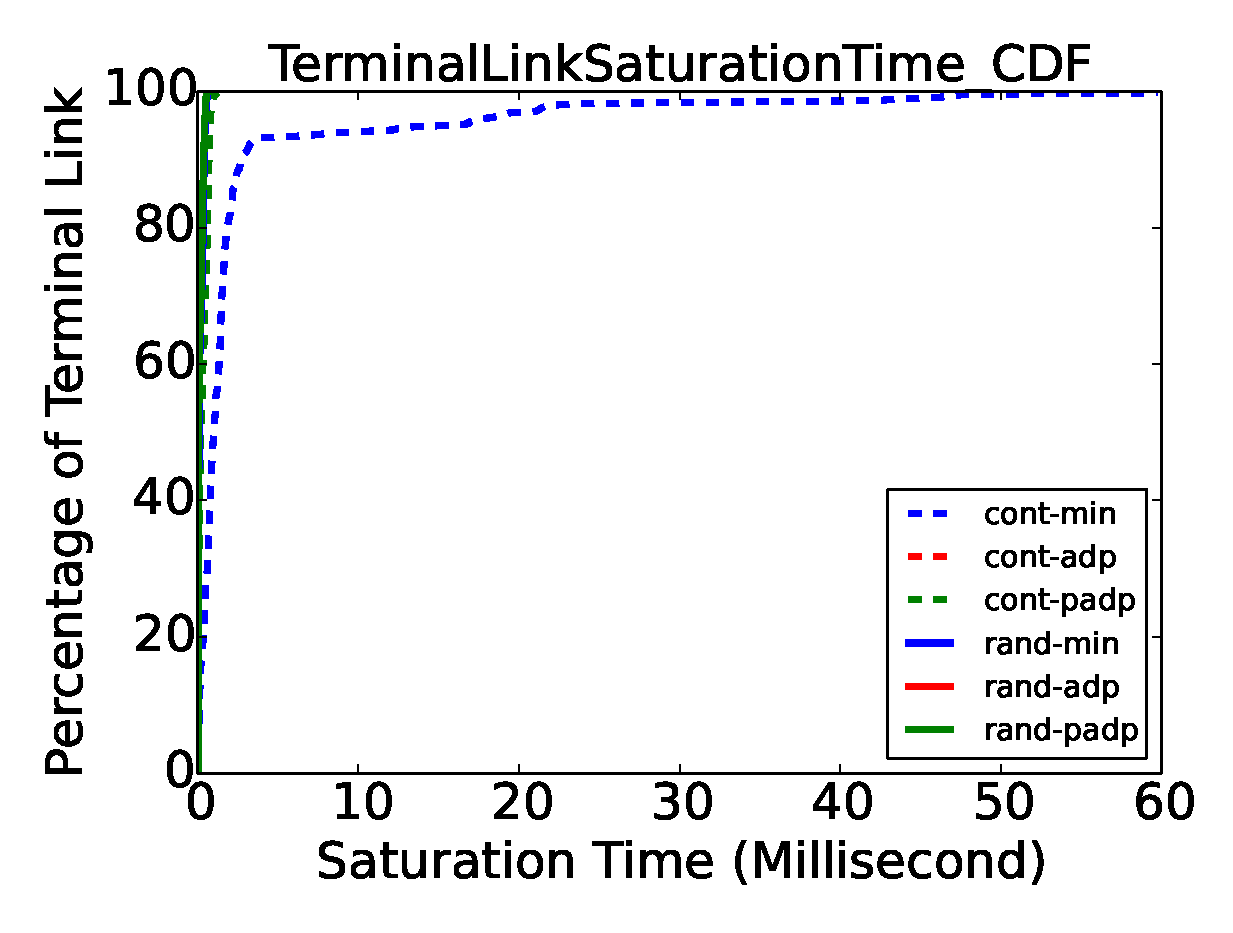
\includegraphics[height=1.8 in]{wkld/tl-stime}
        \caption{Terminal Link Saturation Time}
        \label{fig:terminal-link-stime}
    \end{subfigure}%
    \caption{Aggregate traffic and saturation time for Workload~\Rmnum{1} under the configurations listed in Table~\ref{tab: placement routing configs}. ``CA'' and ``CPA'' have equivalent behavior.}
   \label{fig:wkld-network-traffic-stime}
\end{figure*}


Figure~\ref{fig:wkld-network-traffic-stime} shows the aggregate traffic for terminal links, local and global channels,
as well as the corresponding saturation time for Workload~\Rmnum{1} under the placement and routing configurations summarized in Table~\ref{tab: placement routing configs}.
%explain CM
When contiguous placement is coupled with minimal routing (CM), 
application traffic is confined within the consecutively allocated groups, 
causing congestion on some routers along minimal paths to and from application nodes. 
Both local and global channels experience significant congestion, as applications span multiple groups.
Similarly, the saturation time for both local and global channels are the highest compared with other configurations.
%explain CA and CPA
When contiguous placement is coupled with adaptive (CA) and progressive adaptive (CPA) routing, 
traffic is able to take non-minimal paths via intermediate routers, helping to alleviate congestion along the minimal paths. 
The resulting traffic through the most utilized local and global channels are greatly reduced, 
as shown in Figures~\ref{fig:global-channel-traffic} and~\ref{fig:local-channel-traffic}. 
%\TODO{Traffic is not substantially reduced for local channel traffic}.
Similarly, the corresponding saturation time on local and global channels is also reduced significantly, 
demonstrating the efficacy of adaptive routing in this case. 
%\TODO{How do we explain the similar distribution of traffic on local channels compared to the dissimilar distribution of saturation time?}
For contiguous placement, we see no perceptible difference in behavior between adaptive and progressive adaptive routing.


%Explain RM
In most cases for this study, the random placement policy behaves similarly across routing policies.
Random placement uniformly distributes MPI ranks over the network, 
balancing the resulting traffic load. 
As shown in Figures~\ref{fig:global-channel-traffic} and~\ref{fig:local-channel-traffic}, 
no router experiences an exceptionally high volume of traffic on its local and global channels. 
When random placement is coupled with minimal routing (RM), less traffic is generated on account of
the packets avoiding intermediate forwarding. At the same time, there is still significant congestion on local channels due to the lack of ability of packets to traverse non-minimal routes, falling into the same trap as the contiguous-minimal configuration.
%\TODO{check this}
%Explain RA, RPA
Coupled with (progressive) adaptive routing,
saturation times are effectively minimized on both global and local channels when random placement is in use, 
as shown in Figure~\ref{fig:global-channel-stime} and~\ref{fig:local-channel-stime}. Further, in comparison to contiguous allocations, random allocations result in a more evenly distributed load on the resulting channels, as expected.

% Explain terminal link traffic and busy time
Figures~\ref{fig:terminal-link-traffic} and \ref{fig:terminal-link-stime} are presented for the purpose of symmetry, 
showing the traffic per terminal link as well as the saturation time experienced at each terminal.
The terminal traffic distribution corresponds directly to application traffic, as we are using one MPI rank per node (terminal).
However, saturation times are different, resulting from the aforementioned network behavior. Particularly, contiguous allocations coupled with minimal routing results in a ``long-tail`` distribution of saturation time.

%===========================================================
%from the workload perspective to study the network performance. 
%The efficiency of the workload communication is another perspective to evaluate the network performance. 
%The average communication time spent by all MPI ranks when Workload~\Rmnum{1} is running under different placement and routing configurations shown in Table~\ref{tab:wkld-commtime}. 
%The random placement policy performs comparably with all routing policies (RM, RA and RPA). They outperform all contiguous placement configurations (CM, CA and CPA). The contiguous placement coupled with minimal routing (CM) results in highest communication time. When coupled with (progressive) adaptive routing (CA, CPA), the average communication time can be greatly reduced. When random placement is in use, the workload communication efficiency can be further improved. 
%
%
%\begin{table}[ht]
%\begin{center}
%\caption{Average communication time by all MPI ranks when Workload I is running on the dragonfly network under six different placement and routing configurations.} 
%\label{tab:wkld-commtime}
%\begin{tabular}{l c c c c c c }
%\toprule % Top horizontal line
%\toprule
%&\multicolumn{6}{c}{Placement and Routing Configurations} \\ 
%\cmidrule(l){2-7}
%          & CM & CA & CPA & RM & RA & RPA \\ % Column names row
%\midrule % In-table horizontal line
%Time(ms)  & 476  & 300  & 301  & 255  & 265  & 264  \\ % Content row 1
%
%\midrule % In-table horizontal line
%\bottomrule % Bottom horizontal line
%\end{tabular}
%\end{center}
%\end{table}
%
%
%The random placement can balance the network traffic load by uniformly distribute the traffic. The (progressive) adaptive routing can avoid the hot-spots by redirecting the traffic away from congested area. The network can reach its optimal performance, when random placement coupled with (progressive) adaptive routing are in use. 
%



\subsection{Individual Application Analysis}
\label{sec: workload-1 app analysis}

\begin{figure*}[t!]
    \centering
    \begin{subfigure}[t]{0.32\textwidth}
        \centering
        \includegraphics[height=1.5 in]{wkld/mg/commtime}
        \caption{MultiGrid}
        \label{fig:mg-commtime}
    \end{subfigure}%
    \hspace{1em}%
    \begin{subfigure}[t]{0.32\textwidth}
        \centering
        \includegraphics[height=1.5 in]{wkld/cr/commtime}
        \caption{CrystalRouter}
        \label{fig:cr-commtime}
    \end{subfigure}%
    \hspace{1em}%
    \begin{subfigure}[t]{0.32\textwidth}
        \centering
        \includegraphics[height=1.5 in]{wkld/amg/commtime}
        \caption{AMG}
        \label{fig:amg-commtime}
    \end{subfigure}%
    \caption{Communication time distribution across application ranks in Workload~\Rmnum{1}.}
   \label{fig:apps-commtime}
\end{figure*}

Now that the system-level view has been analyzed, we turn to evaluate the
behavior of each application within Workload~\Rmnum{1}.
Figure~\ref{fig:apps-commtime} shows the communication time distribution across
application ranks for different placement and routing configurations.

The relative behavior of contiguous allocations is roughly similar in all three
applications. Contiguous placement with minimal routing results in poor relative
performance across the board compared to the adaptive routing alternatives.
Given the analyses in Section~\ref{sec: workload-1 network analysis}, this is to
be expected -- the contiguous-minimal configuration results in significant
congestion.

For the MultiGrid and CrystalRouter applications (Figures~\ref{fig:mg-commtime} and
\ref{fig:cr-commtime}, respectively), using random allocation with any routing
method results in performance improvements over contiguous allocations, which is
largely in agreement with the literature (see Section~\ref{sec:related work}).
%\TODO{did previous work make this strong a claim? yes, that's the finding in Nik and Abi's SC papers}. 
The high-radix nature of the
network topology ensures that the benefits from the resulting load balancing
outweigh the costs of extra hops for point-to-point messages.

The AMG application (Figure~\ref{fig:amg-commtime}), however, shows markedly
different behavior when using random allocation. Random allocation with minimal
routing results in worse performance than contiguous-adaptive configurations,
while using adaptive routing results in significant performance regressions. As
this is a counterintuitive result not reached by other works, we investigate
further.

\begin{comment} JJ - doing some reorg, so keeping the old text just in case
Now that the system-level view has been analyzed, we turn to evaluate the behavior of each application within Workload~\Rmnum{1}.
Figure~\ref{fig:apps-commtime} shows the communication time distribution across application ranks for different placement and routing configurations.
As shown in Figure~\ref{fig:mg-commtime}, 
MultiGrid takes the most communication time when it is running with contiguous placement and minimal routing (CM). 
When contiguous placement coupled with adaptive or progressive adaptive routing (CA, CPA) are in use, 
the communication time is significantly reduced. 
Random placement coupled with minimal routing (RM) can make further improvement, 
and reaches the best performance(lowest communication time) when coupled with adaptive and progressive adaptive routing(RA, RPA). 
Due to the variance of data transfer amount among MPI ranks, 
MultiGrid communication time also presents great variation, 
indicating by the long boxes in Figure~\ref{fig:mg-commtime}.

CrystalRouter takes more communication time compared with the other applications because of its high volume of data transfer. 
When it is running with six placement and routing configurations, 
CrystalRouter communication time presents similarly trend as MultiGrid but with little variance, shown in Figure~\ref{fig:cr-commtime}. 


AMG is quite an exception. 
The communication time of AMG running with different placement and routing configuration are shown in Figure~\ref{fig:amg-commtime}.
When contiguous placement is in use, AMG behaves similarly as MultiGrid and CrystalRouter over three routing policies. 
It takes comparable amount of communication time when contiguous placement coupled with adaptive and progressive routing. 
When coupled with minimal routing, the communication time almost doubles. 
The communication time skyrockets when random placement coupled with (progressive) adaptive routing (RPA, RA) are in use. Minimal routing (RM) can mitigate this performance degradation, but still worse than CA and CPA. We observe that when Workload~\Rmnum{1} is running with random placement and (progressive) adaptive routing, 
the performance of MultiGrid and CrystalRouter are significant improved, whereas AMG suffers performance degradation. 
\end{comment}


\begin{figure*}[t]
    \centering
    \begin{subfigure}[t]{0.32\textwidth}
        \centering
        \includegraphics[height=1.8 in]{wkld/mg/lc-traffic}
        \caption{MultiGrid Local Channel Traffic}
        \label{fig:mg-lc-traffic}
    \end{subfigure}\hfill
    \begin{subfigure}[t]{0.32\textwidth}
        \centering
        \includegraphics[height=1.8 in]{wkld/cr/lc-traffic}
        \caption{CrystalRouter Local Channel Traffic}
        \label{fig:cr-lc-traffic}
    \end{subfigure}\hfill
    \begin{subfigure}[t]{0.32\textwidth}
        \centering
        \includegraphics[height=1.8 in]{wkld/amg/lc-traffic}
        \caption{AMG Local Channel Traffic}
        \label{fig:amg-lc-traffic}
    \end{subfigure}\\  
    \centering
   \begin{subfigure}[t]{0.32\textwidth}
        \centering
        \includegraphics[height=1.8 in]{wkld/mg/gc-traffic}
        \caption{MultiGrid Global Channel Traffic}
        \label{fig:mg-gc-traffic}
    \end{subfigure}\hfill
    \begin{subfigure}[t]{0.32\textwidth}
        \centering
        \includegraphics[height=1.8 in]{wkld/cr/gc-traffic}
        \caption{CrystalRouter Global Channel Traffic}
        \label{fig:cr-gc-traffic}
    \end{subfigure}\hfill
    \begin{subfigure}[t]{0.32\textwidth}
        \centering
        \includegraphics[height=1.8 in]{wkld/amg/gc-traffic}
        \caption{AMG Global Channel Traffic}
        \label{fig:amg-gc-traffic}
    \end{subfigure}
   \caption{Aggregate workload traffic for routers serving specific applications. ``CA'' and ``CPA'' have equivalent behavior. More routers are involved in serving each application when random placement is in use, compared to contiguous placement.}
   \label{fig:3app-lc-gc-traffic}
\end{figure*}

% Show the evidence from network level, explain why AMG is different. 

We step back to a network-level system view to identify the culprit behind AMG's
abnormal behavior with random placement. This time, however, we identify the
compute nodes that each MPI rank resides on and the routers that are serving
each application, and analyze the traffic on a per-application basis.  The
results of this experimentation are presented in
Figure~\ref{fig:3app-lc-gc-traffic}. Note that different numbers of routers are
used in the contiguous and random allocation configurations, as each router
serves multiple terminals.

The system behavior with respect to the CrystalRouter application arguably best
matches expectations. Use of contiguous allocations result in a subset of
channels with a significant traffic load while a significant portion are
unused. Use of random allocations result in a comparatively smoother traffic
distribution, with some variation on the margins due to the randomness.

MultiGrid shows roughly similar behavior for contiguous allocations, but
different behavior along the local channels. There is a significant variation in
the traffic distribution on local channels, even with adaptive routing, which
nevertheless has the net effect of reducing the maximal traffic load.

AMG shows a similar level of variation to MultiGrid in this case. However, it
is the least communication-intensive application of the three by a significant
factor. As evidenced by the wide gap between the router traffic in contiguous
and random placement configurations, the routers serving the AMG application
are being utilized by MultiGrid and CrystalRouter, resulting in AMG traffic
contending with traffic of other applications. The net effect, as shown in
Figure~\ref{fig:amg-commtime}, is significant slowdowns for AMG.
We refer to this phenomenon as AMG being ``bullied" by MultiGrid and CrystalRouter.

\subsection{Key Observations}
\label{sec:workload-1-observations}

In summary, based on the simulations presented in Section~\ref{sec: workload-1 network analysis} and \ref{sec: workload-1 app analysis}, we make the following observations.

\emph{System-level performance is significantly improved when random placement and adaptive routing are in use.} 
Random placement can uniformly distribute MPI ranks of application over the network, 
and adaptive routing can redirect the traffic from congested routers to other less busy routers. 
The combination of the two minimizes hot-spots and promotes load-balanced distribution. The resulting increased number of hops per message was not a significant detriment in comparison. This matches what is seen in the literature.

\emph{The performance of communication-intensive jobs in the system improves through use of random allocation policies.}
Both CrystalRouter and MultiGrid, the two most communication-intensive jobs,
saw improved distributions of communication performance when moving to a
random allocation. Again, this matches what is seen in the literature.

\emph{The performance of less communication-intensive jobs in workload regresses when random placement and adaptive routing are in use.} 
AMG in Workload~\Rmnum{1} is ``bullied" by its concurrently running communication-intensive peers, MultiGrid and CrystalRouter.
AMG shares routers and groups with MultiGrid and CrystalRouter under random placement. 
The traffic from MultiGrid and CrystalRouter is (re)directed to the routers that serve AMG, 
slowing down AMG's communication. 
\footnote{We have tried three different congestion ``sensing'' schemes in the literature for adaptive routing~\cite{won-prog-adaptive}. Although there are some variations between the results, none of the congestion sensing scheme prevent the ``bully'' behavior.}

\emph{In contrast, performance consistency of each application is achieved only when contiguous placement and minimal routing are in use.} 
As a corollary to the previous observation, router and group sharing among applications are guaranteed to be prohibited when using contiguous placement with minimal routing (sharing of spare nodes within a group notwithstanding). This renders the ``bully'' behavior moot, though with the downside of significant performance degradation, so such approaches must be carefully considered.
%\TODO{not sure whether to keep this -- we don't really talk about performance consistency in the preceding text. It's a valid observation, though, so it should be somewhere...} 

